\subsection{Algorithmus}\label{subsec:splay-algorithmus}
Ein Splay-Baum ist ein Binärbaum, der beim Einfügen und Suchen von Elementen, diese jeweils an
die Wurzel befördert.
Dieser Vorgang wird Splaying genannt.

\subsubsection{Splaying}
Ähnlich wie beim AVL-Baum wird wieder ein Knoten als Wurzel betrachtet.
Zunächst wird das gesuchte Element an diese Wurzel gebracht.
Dieser Prozess wird anschließend rekursiv auf die verbleibenden Knoten über der Wurzel angewendet,
bis das Element an der Wurzel des kompletten Baumes steht.

Es wird zwischen 3 Fällen unterschieden, die durch den Pfad von der Wurzel zu dem nach oben
zu befördernden Elementes definiert sind.
Alle Fälle haben jeweils ein symmetrisches Paar.
In Abbildung~\ref{fig:splayinCase} ist jeweils eines der Paare dargestellt.
In Klammern ist der symmetrische Fall angegeben.
Die Wurzel \verb|x| ist dabei jeweils die, die nach oben befördert werden soll.
Der Vorgang wird im Entwurf der Methode \nameref{par:splay} (Abschnitt~\ref{par:splay})
weiter ausgeführt.
%\begin{enumerate}
%    \item Zig-Zag: L/L oder R/R
%    \item Zig-Zig: L/R oder R/L
%    \item Zig: L oder R
%\end{enumerate}

\begin{figure}[hbt]
    \centering
    \subfloat[\centering Zig Zig: L/L (R/R)]{
        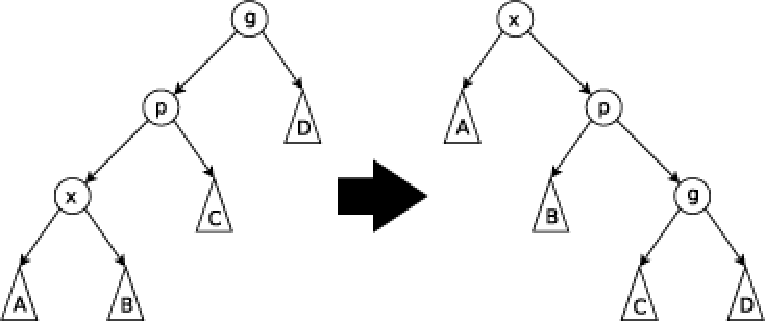
\includegraphics[width = 0.45\textwidth]{img/external/zigzig}\label{fig:splayingCase-zig-zig}}
    \qquad
    \subfloat[\centering Zig Zag: L/R (R/L)]{
        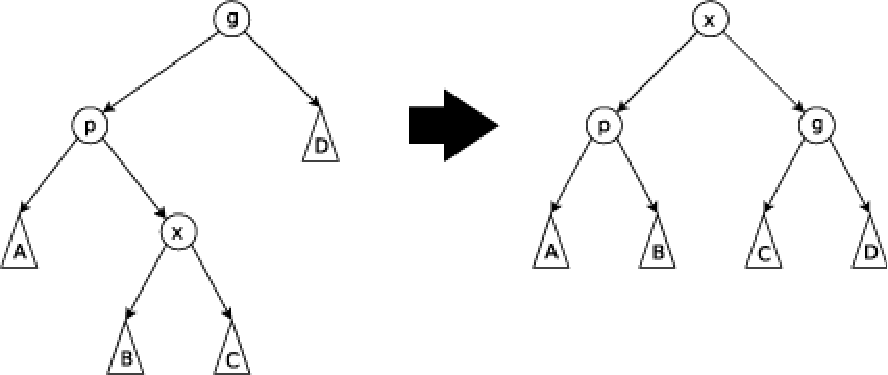
\includegraphics[width = 0.48\textwidth]{img/external/zigzag}\label{fig:splayingCase-zig-zag}}
    \qquad
    \subfloat[\centering Zig: L (R)]{
        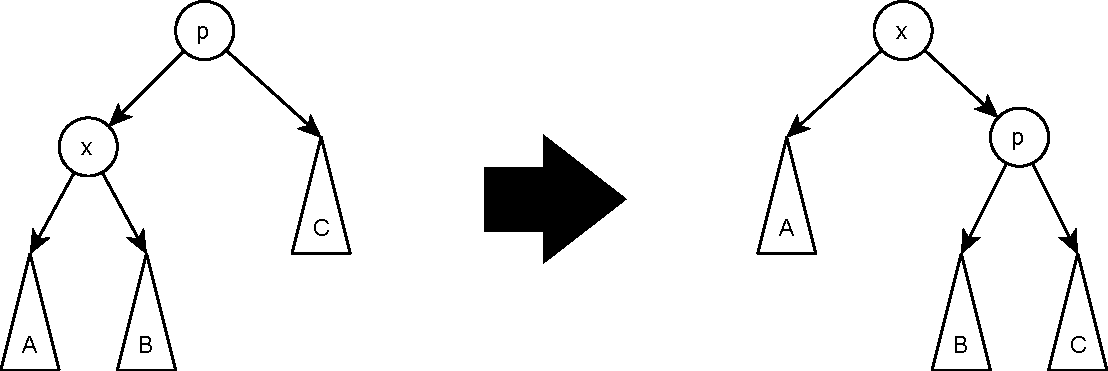
\includegraphics[width = 0.52\textwidth]{img/external/zig}\label{fig:splayingCase-zig}}
    \caption{Splaying Vorgang}\label{fig:splayinCase}
\end{figure}

\subsection{Entwurf}\label{subsec:splay-entwurf}

\subsubsection{InitBT, IsEmptyBT, EqualBT, PrintBT}
Wie beim AVL-Baum kann auch hier die Implementation des Binärbaumes verwendet werden.
Lediglich InitBT wird wieder um das Zurücksetzen der Counter erweitert.
PrintBT ist identisch zu der in Abschnitt~\ref{par:printBT} beschrieben Methode.

\subsubsection{IsBT}
Bei dem AVL-Baum wurde \nameref{par:avl-isBT} um das Überprüfen der AVL-Bedingung erweitert.
So konnte die korrekte Arbeitsweise des AVL-Baumes sichergestellt werden.
Bei dem Splay-Baum lässt sich die Korrektheit vom Splaying jedoch nicht überprüfen, da die
Datenstruktur selber keine Informationen über die Zugriffe auf Elemente speichert.
In \verb|IsBT(BTree)| werden also lediglich die Voraussetzungen des Binärbaumes überprüft,
somit kann die Implementation vom Binärbaum übernommen werden.

\subsubsection{FindBT}\label{par:splay-findBT}
Beim Finden eines Elementes wird dieses an die Wurzel des Baumes befördert.
Dafür wird zunächst top-down das gesuchte Element gefunden, wobei der Pfad
bottom-up hoch gegeben wird.
Als Erstes wird \verb|HERE|, danach \verb|L| oder \verb|R| zurückgegeben.
Beim zweiten Schritt ist das gesuchte Element zwei Elemente entfernt, kann also über zwei
Kanten erreicht werden.
Nun wird die entsprechende Doppelrotation durchgeführt, dies wird in die \nameref{par:splay}
Methode ausgelagert.
Das gesuchte Element steht jetzt an dem Knoten, der gerade als Wurzel betrachtet wird, somit wird
als Pfad \verb|HERE| zurückgegeben.
Dies wird rekursiv fortgeführt, bis die Wurzel des Baumes erreicht wird.
Der Vorgang ist in Abbildung~\ref{fig:splayFind} dargestellt.
\begin{figure}[hbt]
    \centering
    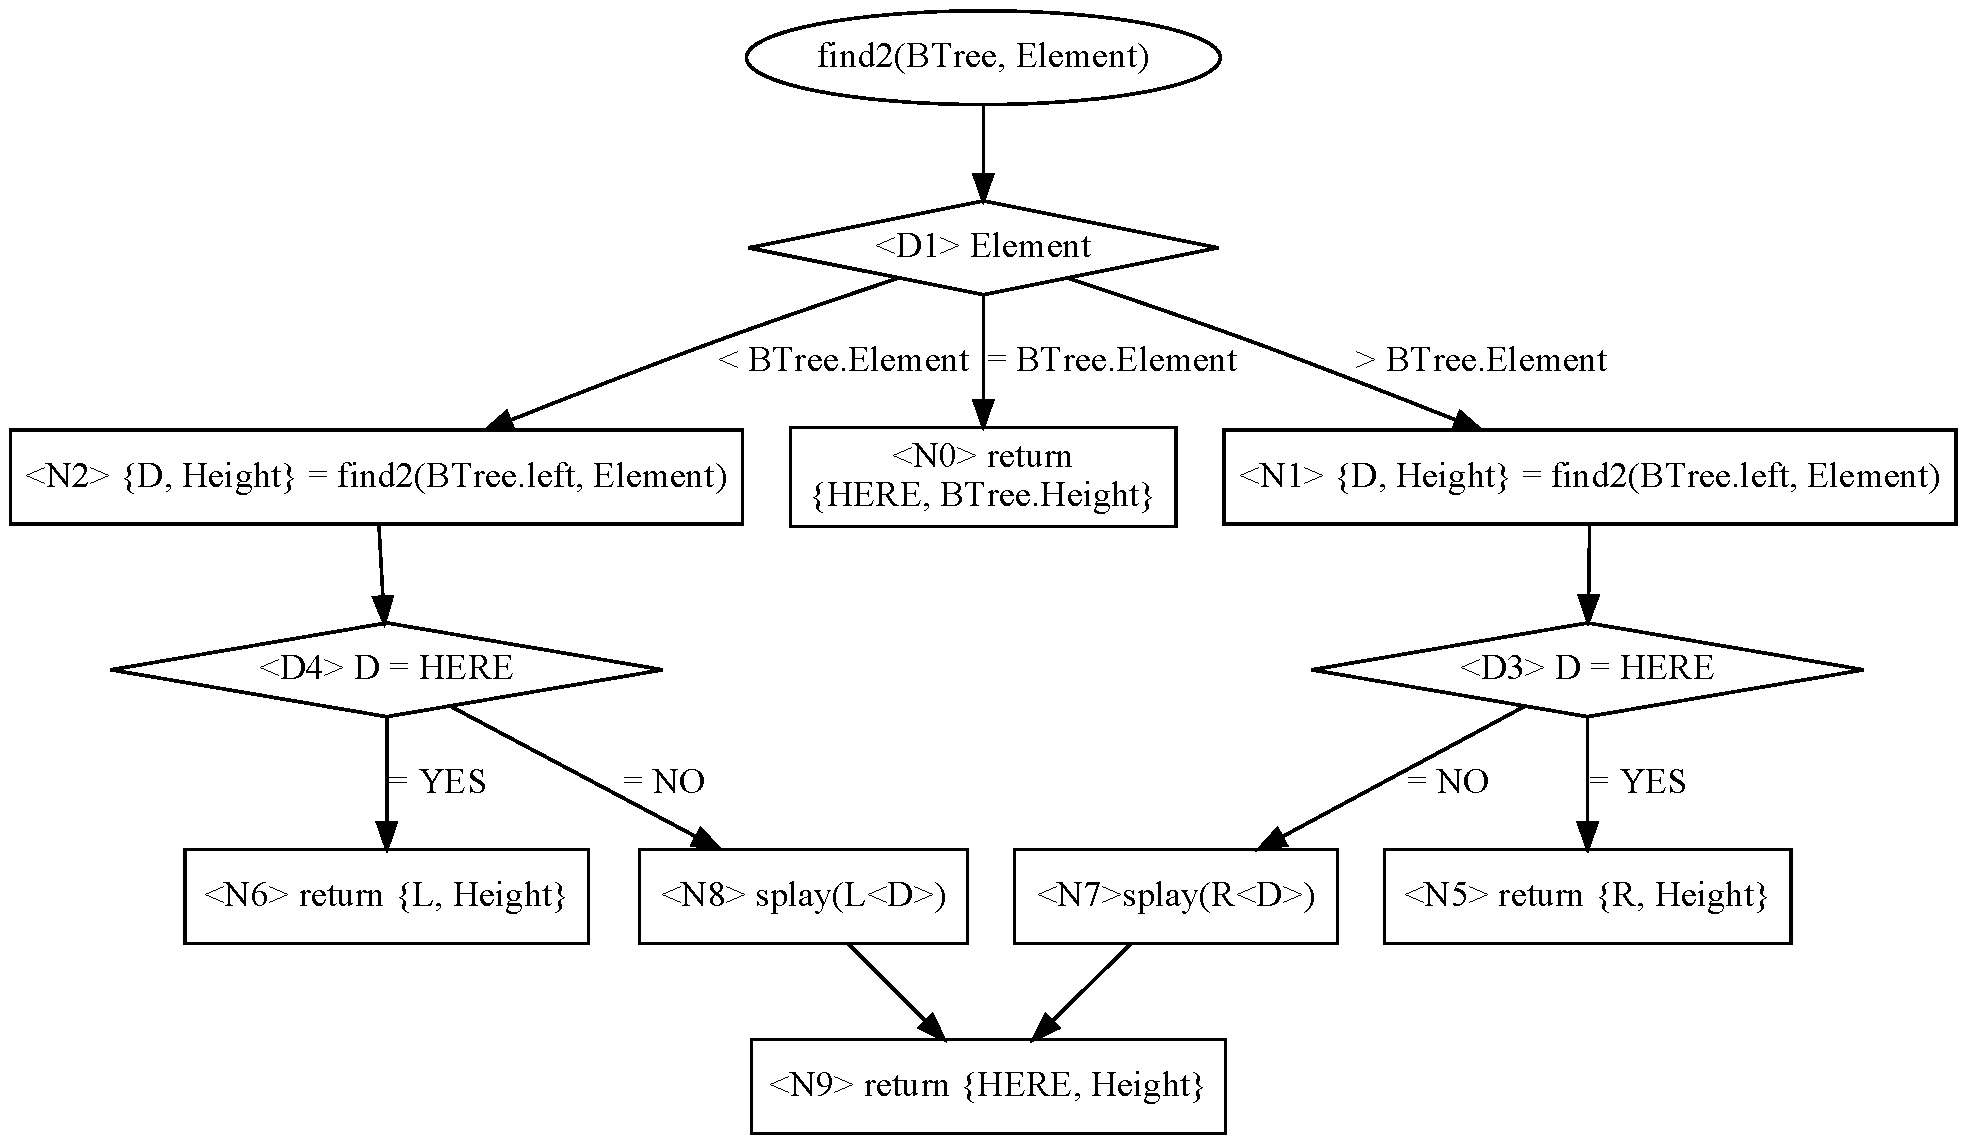
\includegraphics[scale = 0.35]{img/gv/splayFind2}
    \caption{FindBT}
    \label{fig:splayFind}
\end{figure}

In der Abbildung ist der Fall, dass das gesuchte Element nicht im Baum vorhanden ist, präteriert.
Hierfür wird der Pfad als \verb|NOTFOUND| zurückgegeben.
Falls bei der Überprüfung dessen \verb|NOTFOUND| vorliegt, wird wiederum \verb|HERE|
zurückgegeben, was dazu führt, dass das zuletzt aufgerufene Element zur Wurzel wird \verb|<R1>|.

Da immer zwei Nachfolger betrachtet werden, ist es möglich, dass am Ende das gesuchte Element
am linken oder rechtem Kind vom Wurzelknoten steht.
Um dies zu überprüfen, wird die eben beschriebene Methode in eine Wrapper-Methode umhüllt.
Dort kann getestet werden, ob am Ende \verb|HERE| zurückgegeben wurde.
Falls dies der Fall ist, wird ein Zig (Einfachrotation) ausgeführt.
Anschließend steht das gesuchte Element an der Wurzel.
Dies ist in Abbildung~\ref{fig:splayFind2} dargestellt.
\begin{figure}[hbt]
    \centering
    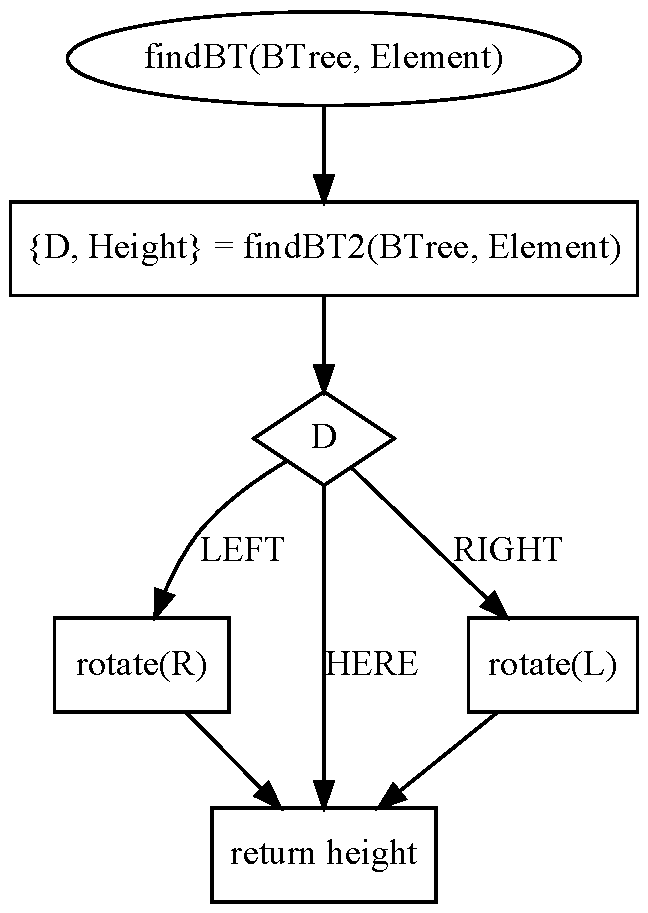
\includegraphics[scale = 0.35]{img/gv/splayFind}
    \caption{FindBT Wrapper}
    \label{fig:splayFind2}
\end{figure}
Diese Operation ist in allen Methoden zu implementieren und wird in den Entwurf dieser nicht
explizit betrachtet.

\subsubsection{Splay}\label{par:splay}
Die Splay Methode bekommt einen Baum und einen Pfad \(P \in \{LL, RR, LR, RL\}\) übergeben,
welcher angibt, welcher Splaying Fall vorliegt.
Es wird eine Fallunterscheidung über den Pfad gemacht, welche die Abfolge der Rotationen bestimmt.
Diese sind wie beim AVL Baum zu implementieren.
\begin{itemize}
    \item LL → Rechtsrotation auf Wurzel → Rechtsrotation auf neue Wurzel. \verb|<R1>|
    \item RR → Linksrotation auf Wurzel → Linksrotation auf neue Wurzel. \verb|<R2>|
    \item RL → Rechtsrotation auf rechtes Kind → Linksrotation auf Wurzel. \verb|<R3>|
    \item LR → Linksrotation auf linkes Kind → Rechtsrotation auf Wurzel. \verb|<R4>|
\end{itemize}

\subsubsection{FindTP}
Alternativ kann beim Finden eines Elementes dieses nur um einen Knoten nach oben bewegt werden.
Zunächst wird das Element gefunden, anschließend eine Zig-Operation durchgeführt.
Um dies zu realisieren, wird, sobald das gesuchte Element gefunden wurde, ein Flag zurückgegeben,
welches signalisiert, dass rotiert werden soll \verb|<R1>|.
Wenn beim Überprüfen des Rückgabewertes das Flag gesetzt ist, wird in die entsprechende Richtung
rotiert \verb|<R2>|.
Somit wird das Element nur um eine Ebene nach oben gegeben, anschließend nicht mehr zurückgegeben
wird \verb|<R3>|.
Falls ein Element nicht gefunden wird, wird \verb|NOTFOUND| zurückgegeben \verb|<R4>|, beim
Überprüfen des Pfades wird daraufhin \verb|HERE| zurückgeben \verb|<R5>|, was dazu führt, dass
wieder genau einmal rotiert wird.

\subsubsection{InsertBT}
Beim Einfügen eines Elementes wird dieses an die Wurzel befördert.
Dies kann dadurch realisiert werden, dass das Element zunächst wie bei einem Binärbaum
eingefügt, anschließend mithilfe von \nameref{par:splay-findBT} an die Wurzel befördert wird.
Diese Implementation hat den Nachteil, dass der Baum insgesamt zweimal durchlaufen wird.
Zur Optimierung werden, beide Schritte in einem Durchlauf durchgeführt: Zunächst top-down
das Element einfügen \verb|<R1>|, dann, mithilfe von Rotationen, bottom-up das Element zur Wurzel
bringen \verb|<R2>|.
Dabei ist letzteres wie bei \nameref{par:splay-findBT} zu realisieren,
die Höhe muss dabei nicht zurückgegeben werden.
Außerdem muss das \verb|NOTFOUND| nicht zurückgegeben werden, da dieser Fall hier nicht auftritt.
Stattdessen wird nach dem Einfügen \verb|HERE| zurückgegeben, damit dieses Element gesplayt wird
\verb|<R3>|.

\subsubsection{DeleteBT}
Bei deleteBT wird ein Element als Erstes mit \nameref{par:splay-findBT} an die Wurzel befördert
\verb|<R1>|.
Dieses wird gelöscht, nun bleiben zwei Teilbäume, übrig, welche mit \nameref{par:joinbt} zu einem
zusammengeführt werden \verb|<R2>|.
Wenn ein Element nicht gefunden wird, wird das zuletzt besuchte Element gesplayt, dies wird wie
in \nameref{par:splay-findBT} (Abschnit~\ref{par:splay-findBT}) realisiert.

\subsubsection{JoinBT}\label{par:joinbt}
Um zwei Bäume zu einem zusammenzuführen wird zunächst das größte Element des linken Teilbaumes
gesplayt \verb|<R1>|, somit hat die neue Wurzel kein rechtes Kind, da es das größte Element des
Baumes ist.
Der rechte Teilbaum wird jetzt als rechtes Kind der neuen Wurzel gesetzt \verb|<R2>|.

\subsection{Aufgaben}\label{subsec:aufgaben2}

\subsubsection{Aufgabe 2.5 - Analysieren beispielhafter Bäume}
Beispielhafte Bäume werden mit der zur verfügung gestellten Methode\\
\verb|analysesBT:test(<Anzahl Elemente>)| analysiert.

\subparagraph{100 Elemente}
Ein Aufruf mit 100 Elementen ergibt folgende Ausgabe:
\begin{verbatim}
> analysesBT:test(100).
Ausgaben beziehen sich auf die Rahmenbedingungen von AVL-Bäumen.
Bei gegebener Höhe 17:
         minimale Anzahl Knoten: 4180.
         maximale Anzahl Knoten: 131071
Bei gegebener Anzahl an Knoten 100:
         minimale Höhe: 6.
         maximale Höhe: 9
Durchschnittliche Balancefehler: 2.19
         maximaler Balancefehler: 10.
\end{verbatim}

\subparagraph{1000 Elemente}
Ein Aufruf mit 1000 Elementen ergibt folgende Ausgabe:
\begin{verbatim}
> analysesBT:test(1000).
Ausgaben beziehen sich auf die Rahmenbedingungen von AVL-Bäumen.
Bei gegebener Höhe 25:
         minimale Anzahl Knoten: 196417.
         maximale Anzahl Knoten: 33554431
Bei gegebener Anzahl an Knoten 1000:
         minimale Höhe: 9.
         maximale Höhe: 14
Durchschnittliche Balancefehler: 1.97
         maximaler Balancefehler: 18.
\end{verbatim}

An den Ausgaben ist zu erkennen, dass die Bäume im Vergleich zu AVL-Bäumen deutlich schlechter
balanciert sind.
Bei beiden Ausgaben ist der durchschnittliche Balancefehler ca. 2, wobei dieser bei den
AVL-Bäumen nur bei ca. 0.3 lag.
Außerdem überschreitet die Höhe vom Splay-Baum im ersten Beispiel die maximale Höhe eines AVL-Baumes
um 100 Prozent.
Hierdurch wird ersichtlich, dass ein Splay-Baum für Zufällige Lese- und Schreiboperationen eine
schlechtere Charakteristik aufzeigt.

\subsubsection{Aufgabe 2.6 - Prüfen der Strategie anhand von Bildern}
Zum Prüfen der Korrektheit der Strategie werden kleine Bäume mithilfe von printBT ausgegeben.
In Abbildung~\ref{fig:splay-base} ist der Ausgangsbaum dargestellt.
Alle folgenden Operationen werden auf diesem Baum ausgeführt.

\paragraph{Im Baum vorhandene Elemente}
In Abbildung~\ref{fig:splay-del4} wurde die 4 gelöscht.
Der Vaterknoten der 4 ist die 3 gewesen, somit wurde diese gesplayt und steht nun an der Wurzel.

In Abbildung~\ref{fig:splay-findbt4} wurde die \verb|FindBT(4)| auf den Ausgangsbaum angewandt,
die 4 wurde gesplayt und steht jetzt an der Wurzel.

In Abbildung~\ref{fig:splay-findtp4} wurde die \verb|FindTP(4)| auf den Ausgangsbaum angewandt.
Die 4 wurde um eine Position gesplayt.

In Abbildung~\ref{fig:splay-insert10} wurde die 10 eingefügt, diese wurde an die Wurzel gesplayt.

\begin{figure}[hbt]
    \centering
    \subfloat[\centering Ausgangsbaum]{
        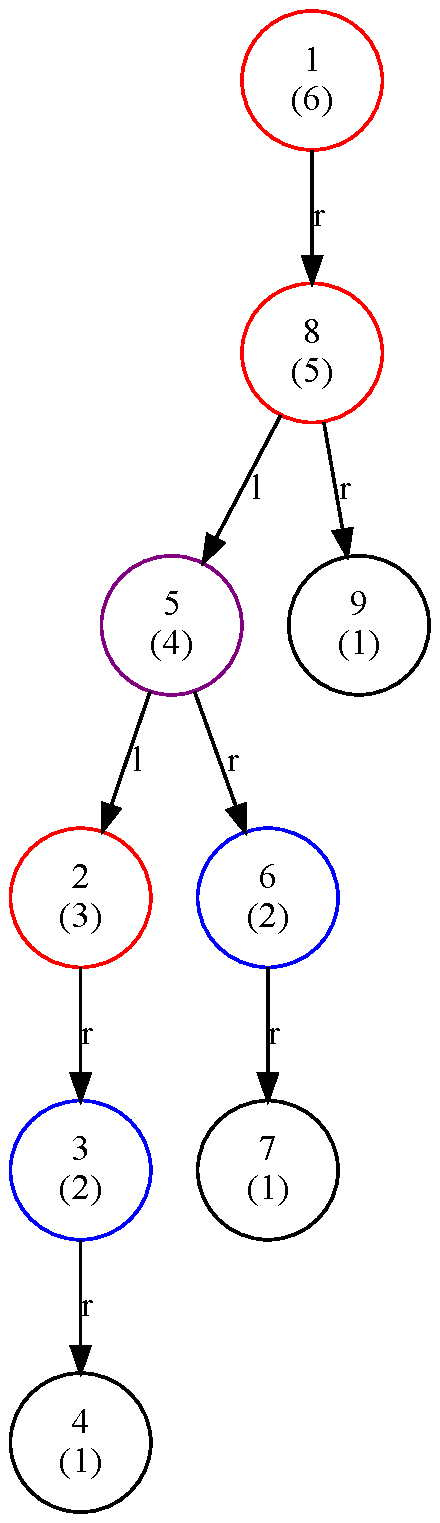
\includegraphics[scale = 0.32]{img/gv/aufg2_6}\label{fig:splay-base}}
    \qquad
    \subfloat[\centering Delete 4]{
        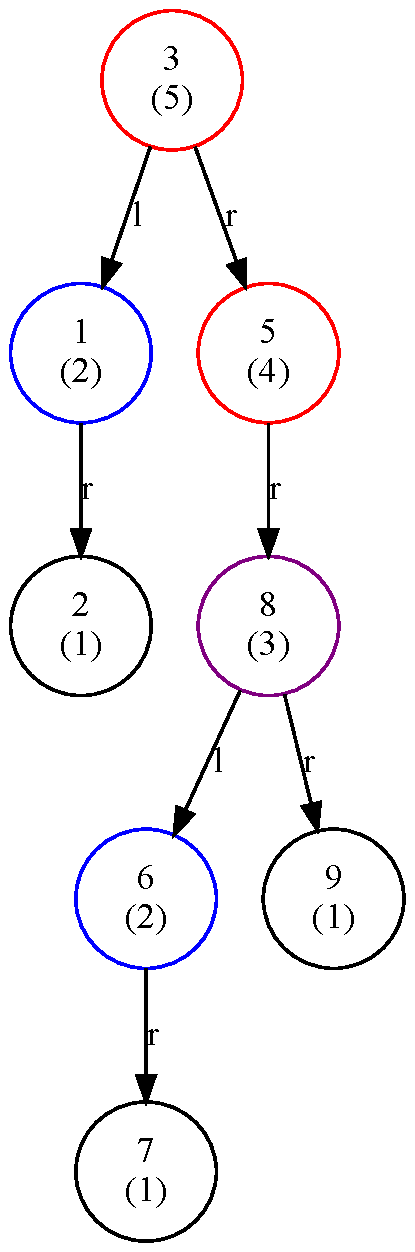
\includegraphics[scale = 0.32]{img/gv/aufg2_6_Delete4}\label{fig:splay-del4}}
    \qquad
    \subfloat[\centering FindBT 4]{
        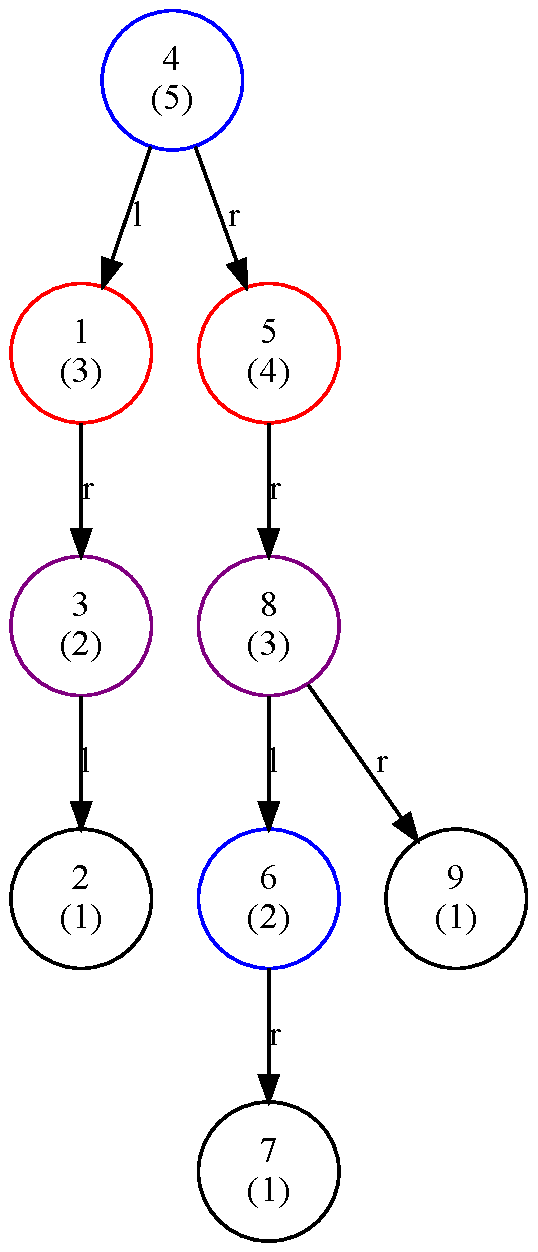
\includegraphics[scale = 0.32]{img/gv/aufg2_6_FindBT4}\label{fig:splay-findbt4}}
    \qquad
    \subfloat[\centering FindTP 4]{
        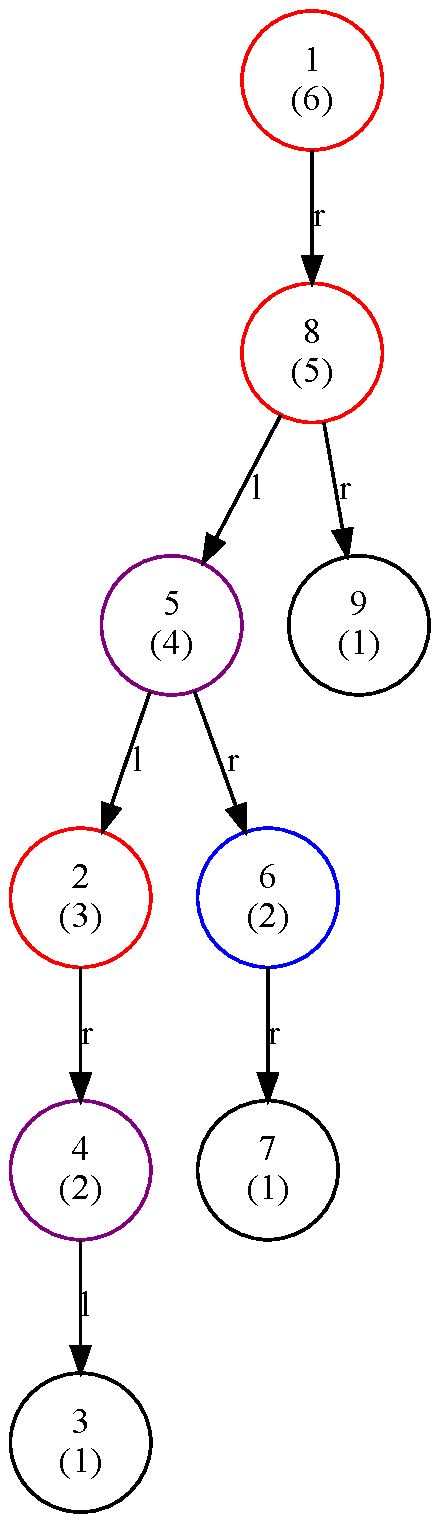
\includegraphics[scale = 0.32]{img/gv/aufg2_6_FindTP4}\label{fig:splay-findtp4}}
    \caption{Bilder der Splaying-Strategie - vorhandene Elemente}\label{fig:splay}
\end{figure}

\paragraph{Im Baum nicht vorhandene Elemente}

In Abbildung~\ref{fig:splay-findbt99} und Abbildung~\ref{fig:splay-delete99} wurde jeweils die
99 gesucht bzw gelöscht.
Da die 99 nicht existiert wurde der Vaterknoten (9) gesplayt und steht anschließend an der Wurzel.

In Abbildung~\ref{fig:splay-findtp99} wurde die \verb|FindTP(99)| auf den Ausgangsbaum angewandt.
Hier wurde die 9 um eine Position gesplayt.

\begin{figure}[hbt]
    \centering
    \subfloat[\centering Insert 10]{
        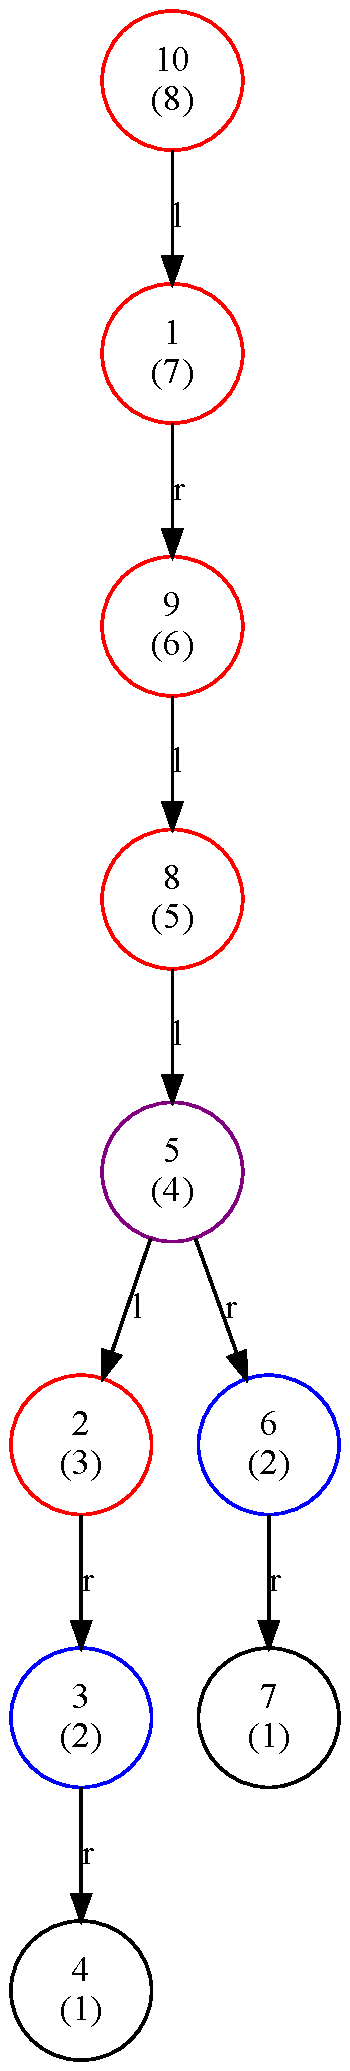
\includegraphics[scale = 0.32]{img/gv/aufg2_6_Insert10}\label{fig:splay-insert10}}
    \qquad
    \subfloat[\centering FindTP 99]{
        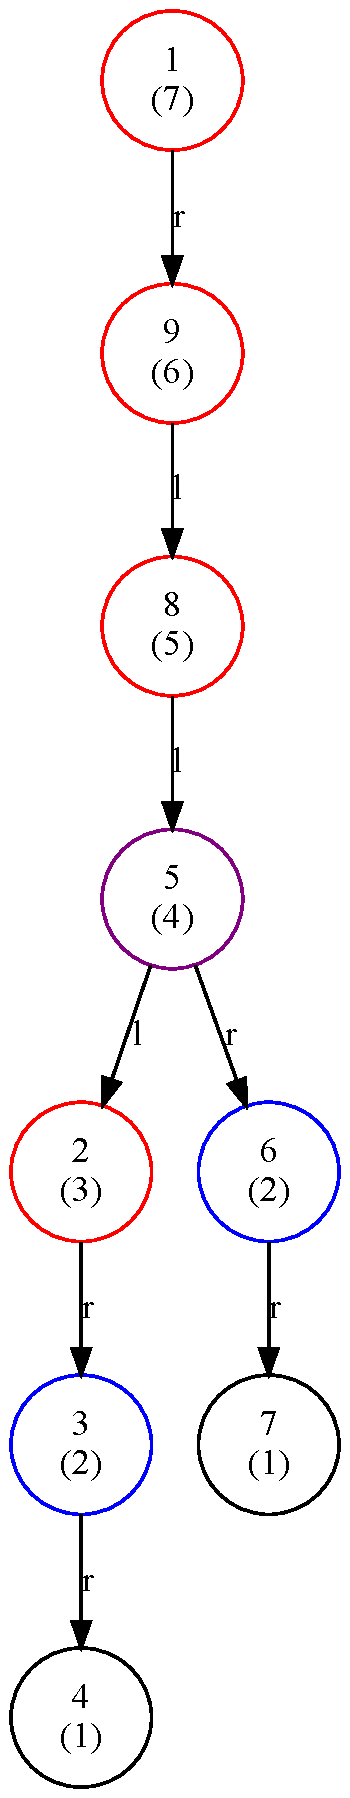
\includegraphics[scale = 0.32]{img/gv/aufg2_6_FindTP99}\label{fig:splay-findtp99}}
    \qquad
    \subfloat[\centering Delete 99]{
        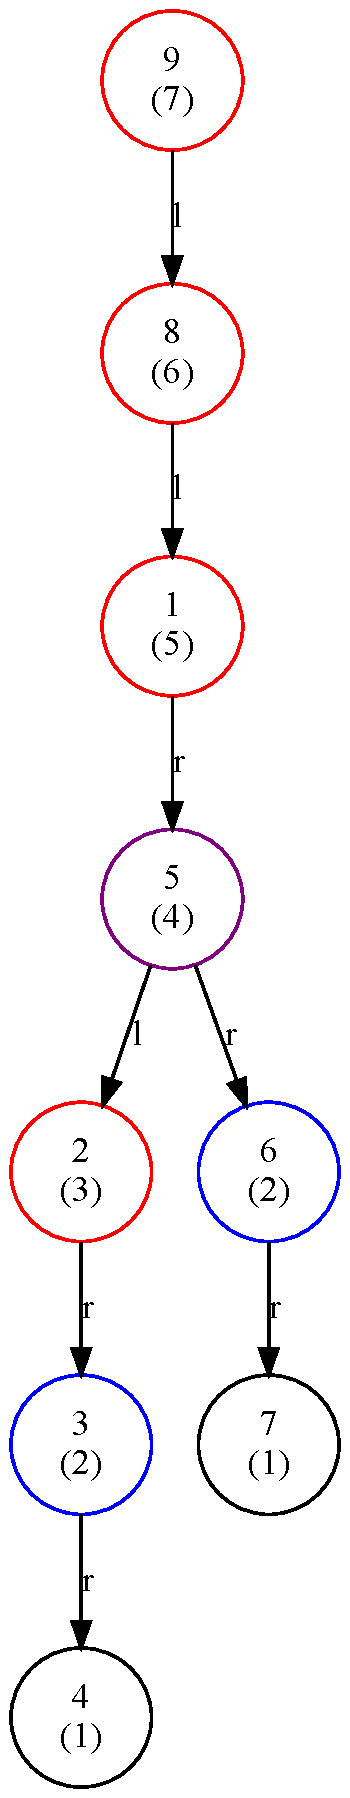
\includegraphics[scale = 0.32]{img/gv/aufg2_6_Delete99}\label{fig:splay-delete99}}
    \qquad
    \subfloat[\centering FindBT 99]{
        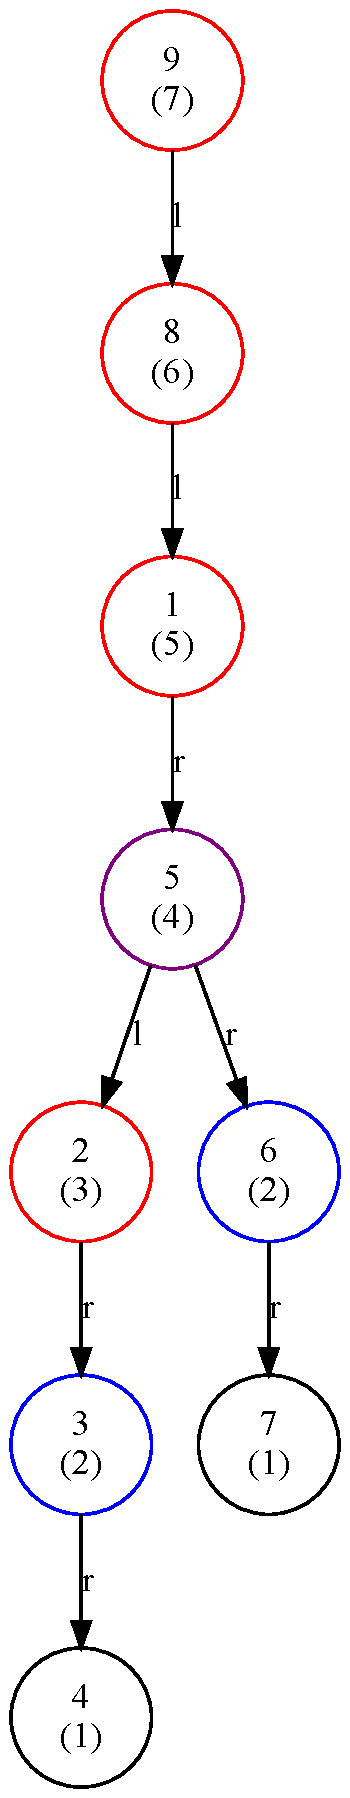
\includegraphics[scale = 0.32]{img/gv/aufg2_6_FindBT99}\label{fig:splay-findbt99}}
    \caption{Bilder der Splaying-Strategie - nicht vorhandene Elemente}\label{fig:splay2}
\end{figure}
